% Intended LaTeX compiler: pdflatex
\documentclass[10pt,a4paper,UTF8]{article}
\usepackage{zclorg}
\author{张朝龙}
\date{}
\title{练习:对偶}
\hypersetup{
 pdfauthor={张朝龙},
 pdftitle={练习:对偶},
 pdfkeywords={},
 pdfsubject={},
 pdfcreator={Emacs 25.0.50.1 (Org mode 9.0.5)},
 pdflang={English}}
\begin{document}

\maketitle
\tableofcontents
\titlepic{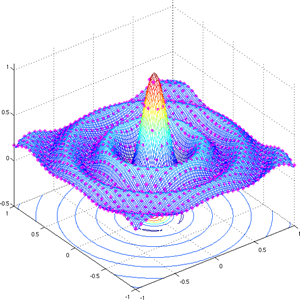
\includegraphics[scale=0.25]{../../img/sinc.PNG}}

\section{3.F.1}
\label{sec:orgdd9d429}


\begin{problem}
解释为什么每个线性泛函或者是满的或者是零映射
\end{problem}

\begin{answer}
\(V\)上的线性泛函是从\(V\)到\(\mathbf{F}\)的线性映射,也就是说,线性泛函是\(\mathcal{L}(V, \mathbf{F})\)中的元素。因为\(\mathbf{F}\)中任何一个非零元素都是\(\mathbf{F}\)的基,所以对于任何\(\varphi\in \mathcal{L}(V, \mathbf{F})\)都有\(\varphi(v)\)属于\(\mathbf{F}\)中的元素。由于\(v\)的任意性,当\(\varphi(v) = 0\)时,则有\(\varphi = 0\),否则\(\varphi(v)\neq 0\)。

我们可以从维度的观点来解释这个问题。因为\(\dim \mathbf{F} = 1\)。若\(\dim range(V) = 0\),则\(\varphi = 0\),若\(\dim rangeV = 1\),则\(\dim range V = \dim \mathbf{F}\). 又因为\(\dim range(V) \leq \dim \mathbf{F} = 1\),所以满射或者零映射是所有的场景。
\end{answer}

\section{3.F.2}
\label{sec:org59e37eb}


\begin{problem}
给出\(\mathbf{R}^{[0,1]}\)上三个不同的线性泛函的例子。
\end{problem}

\begin{answer}
\begin{enumerate}
\item \(\varphi: \mathbf{R} \rightarrow \mathbf{R}\), \(\varphi(x) = x\)
\end{enumerate}
\end{answer}

\section{3.F.3}
\label{sec:org1f29713}


\begin{problem}
设\(V\)是有限维的,\(v\in V\)且\(v \neq 0\),证明存在\(\varphi\in V^{'}\)使得\(\varphi(v) = 1\)
\end{problem}

\begin{answer}
理解题目,\(V^{'}= \mathcal{L}(V, \mathbf{F})\)。从第一题我们知道:线性泛函要么是满的要么是零映射。又因为\(v\neq 0\),所以\(V^{'}\)中的元素都是满的。

特别的,我们把\(v\)扩展成\(V\)的对偶基\(v,v_{2},\ldots ,v_{n}\),则有\(V^{'}\)中的对偶基\(\varphi_{1},\varphi_{2},\ldots ,\varphi_{n}\),则有:
\begin{equation}
\label{eq:1}
\varphi_{k}(v) =
\begin{cases}
1 & k = 1  \\
0 & k\neq 1
\end{cases}
\end{equation}

从一个非零向量扩展出一个基是一个总要的技巧。对偶基的定义也要牢牢掌握。
\end{answer}

\section{3.F.4}
\label{sec:org96bfa99}


\begin{problem}
设\(V\)是有限维的,\(U\)是\(V\)的子空间使得\(U\neq V\),证明存在\(\varphi\in V^{'}\)使得对每个\(u\in U\)有\(\varphi(u) = 0\)但\(\varphi \neq 0\)
\end{problem}

\begin{answer}
因为\(U\)是\(V\)的子空间且\(V\neq U\),我们知道\(\dim V >  \dim U\),又因为\(\dim U + \dim U^{0} = \dim V\),则有\(\dim U^{0} = \dim V - \dim U > 0\),所以\(\dim U^{0} \neq {0}\) 所以在零化子空间中存在非零的线性泛函。
\end{answer}
\section{3.F.5}
\label{sec:orgf360eec}


\begin{problem}
设\(V_{1},\ldots ,V_{m}\)均为向量空间。证明\((V_{1}\times \ldots \times V_{m})^{'}\)和\(V_{1}^{'}\times \ldots \times V_{m}^{'}\)是同构的向量空间。
\end{problem}

\begin{answer}
因为\[\dim (V_{1}\times \ldots \times V_{m})^{'} = \dim (V_{1}\times \ldots \times V_{m})\]而\[ \dim (V_{1}\times \ldots \times V_{m}) = \sum_{i=1}^{m}\dim V_{i}\]

另一方面\[\dim V_{1}^{'}\times \ldots \times V_{m}^{'} = \sum_{i=1}^{m}\dim V_{i}^{'}\] 又因为\[\dim V_{i}^{'} = \dim V_{i},\forall i\]

所以\[\dim (V_{1}\times \ldots \times V_{m})^{'} = \dim V_{1}^{'}\times \ldots \times V_{m}^{'}\]命题得证。
\end{answer}

\section{3.F.6}
\label{sec:org8bcec9f}


\begin{problem}
设\(V\)是有限维的,\(v_{1},\ldots ,v_{m}\in V\),定义线性映射\(\Gamma:V^{'}\rightarrow \mathbf{F}^{m}\)如下:\[\Gamma(\varphi) = (\varphi(v_{1}), \ldots ,\varphi(v_{m}))\]
\begin{enumerate}
\item 证明:\(v_{1},\ldots ,v_{m}\)张成\(V\)当且仅当\(\Gamma\)是单的。
\item 证明\(v_{1},\ldots ,v_{m}\)线性无关当且仅当\(\Gamma\)是满的。
\end{enumerate}
\end{problem}

\begin{answer}
我们先证明第一个命题:

如果\(v_{1},\ldots ,v_{m}\)张成\(V\),那么\(\Gamma(\varphi) = 0\),即\(\varphi\in null \Gamma\)意味着:\[\varphi(v_{1}) = \ldots = \varphi(v_{m}) = 0\]
另外从\(v_{1},\ldots ,v_{m}\)张成\(V\),我们还可以推出,对于任何\(v\in V\),都有\(\exists a_{i}\in \{1,\ldots ,m\}\),使得:\[v= a_{1}v_{1}+\ldots + a_{m}v_{m}\]对上式两端进行\(\varphi\)映射,则有:
\begin{equation}
\label{eq:2}
\varphi(v) = a_{1}\varphi(v_{1}) + \ldots + a_{2}\varphi(v_{m}) = 0
\end{equation}
也就是说,对于\(V\)中的任何一个元素\(v\),都有\(\varphi(v) = 0\),这样的映射\(\varphi\)叫做零映射。所以有\(\Gamma\)的零空间中的任何一个元素都是\(0\),即有\(null\Gamma = 0\),所以\(\Gamma\)是单射。

另一方面:我们从\(\Gamma\)是单射推出\(v_{1},\ldots ,v_{m}\)张成\(V\)。这里我们采用反证法:假设\(\Gamma\)是单射,但是\(v_{1},\ldots ,v_{m}\)不张成\(V\),则有\(U = span(v_{1},\ldots ,v_{m})\)是\(V\)的子集,并且\(U\neq V\)。我们知道\(\dim U + \dim U^{0} = \dim V\),因为\(U\neq V \rightarrow \dim U \neq \dim V\),所以\(\dim U^{0} > 0\),所以\(\exists \varphi \in V^{'},\varphi\neq 0\),满足\(\varphi(v_{1}) = \ldots =\varphi(v_{m}) = 0\),所以\(\varphi \in null \Gamma\)这与\(\Gamma\)是单射矛盾。所以,必有\(\Gamma\)是单射推出\(v_{1},\ldots ,v_{m}\)张成\(V\)。
\end{answer}

\begin{answer}
接下来证明第二个命题:

如果\(v_{1},\ldots ,v_{m}\)是线性独立的,那么对于任何\(f_{1},\ldots ,f_{m}\in \mathbf{F}^{m}\),存在一个映射\(\varphi \in V^{'}\) 满足:
\[\varphi(v_{i}) = f_{i},i=1,\ldots ,m\]
那么根据\(\Gamma\)的定义有:\[\Gamma(\varphi) = (f_{1},\ldots ,f_{m})\] 说明\(\Gamma\)是满射。因为对于任意的\(f_{1},\ldots ,f_{m}\)都可以找到一个映射,说明\(range(\Gamma) = \mathbf{F}^{m}\)


对于任意的\(f_{1},\ldots ,f_{m}\)这个映射的存在是有依据的,我们之前就证明过一个命题。现在把这个命题重述如下:

设\(v_{1},\ldots ,v_{m}\)是\(V\)的基,\(w_{1},\ldots ,w_{m}\in W\),则存在唯一一个线性映射\(T:V\rightarrow W\)使得对于任意\(j=1,\ldots ,n\)都有:\[Tv_{j}= w_{j}\]这个定理的证明见 \href{linear-map-on-vector-space.org}{线性映射} 一文。这个定理说明线性映射可以根据其在一个基上的取值来构造,而唯一性表明一个线性映射完全由其在基上的取值确定。时至今日,我对3.5的这个定理有了更深的理解。

接下来我们证明另一个方面,如果\(\Gamma\)是满射,我们要证明\(v_{1},\ldots ,v_{m}\)是线性独立的。假设\(v_{1},\ldots ,v_{m}\)是线性相关的。注意我们在用反证法了,我们希望推出矛盾。存在不全为零的一组数\(k_{1},\ldots ,k_{m}\in \mathbf{F}\)满足:\[k_{1}v_{1} + ... + k_{m}v_{m} = 0\] 假设\(k_{i}\neq 0\),那么\(v_{i}\)可以写成\(v_{1},\ldots ,v_{i-1},v_{i+1},\ldots ,v_{m}\)的线性组合。所以第\(i\)个元素为\(1\),其他元素为\(0\)的向量\((0,\ldots ,0,1,0,\ldots ,0)\)不在\(range \Gamma\)中。所以\(\Gamma\)不是满射,所以\(v_{1},\ldots ,v_{m}\)是线性独立的。

为什么第\(i\)个元素为\(1\),其他元素为\(0\)的向量\((0,\ldots ,0,1,0,\ldots ,0)\)不在\(range \Gamma\)中?我们这里做一下详细的说明。

假设第\(i\)个元素为\(1\),其他元素为\(0\)的向量\((0,\ldots ,0,1,0,\ldots ,0)\)在\(\Gamma\)中,那么存在一个映射\(\varphi\in V^{'}\),使得:\[\varphi(v_{j}) = 0, \varphi(v_{i}) = 1,j = 1,\ldots ,i-1,i+1,\ldots ,m\] 这意味着\(\varphi(v) = 0\),如果\(v\)是\(v_{1},\ldots ,v_{i-1},v_{i+1},\ldots ,v_{m}\)的线性组合。因为我们假设\(v_{1},\ldots ,v_{m}\)是线性相关的并且\(v_{i}\)可以用其他向量的线性组合来表示,所以\(\varphi(v_{i}) = 0\)。但是我们有\(\varphi(v_{i}) = 1\),矛盾。\(\Gamma\)不是满射。这意味着\(v_{1},\ldots ,v_{m}\)是不可能是线性相关的。

这个问题在证明的过程中,我有几个知识点没有掌握:

\begin{enumerate}
\item 线性映射可以通过这个线性映射在一个基上的取值来构造。
\item 反证法中寻找有利于结论的特例
\end{enumerate}
\end{answer}
\section{3.F.7}
\label{sec:org9a7b87f}


\begin{problem}
设\(m\)是正整数。证明\(\mathcal{P}_{m}(\mathbf{R})\)的基\(1,x,\ldots ,x^{m}\)的对偶基是\(\varphi_{0},\ldots ,\varphi_{m}\)其中\(\varphi_{j}(p) = \frac{p^{(j)}(0)}{j!}\),\(p^{(j)}\)表示\(p\)的\(j\)次导数,\(p\)的\(0\)次导数规定\(p\)
\end{problem}

\begin{answer}
根据对偶基的定义,假设\(v_{1},\ldots ,v_{m}\)是\(V\)的基,则其对偶基\(\varphi_{1},\ldots ,\varphi_{m}\in V^{'}\)满足:
\begin{equation}
\label{eq:3}
\varphi_{j}(v_{k}) =
\begin{cases}
1 & k=j \\
0 & k\neq j
\end{cases}
\end{equation}

对于题目中的对偶基,我们只需要按照定义来验证就可以,对于:
\begin{equation}
\label{eq:4}
\varphi_{j}(v_{k}) = \frac{(x^{k})^{(j)}}{j!}
\begin{cases}
1 & k = j \\
0 & k\neq j
\end{cases}
\end{equation}

结论是显然的。
\end{answer}
\section{3.F.8}
\label{sec:org060de27}


\begin{problem}
设\(m\)是正整数。

\begin{enumerate}
\item 证明\(1,x-5,\ldots ,(x-5)^{m}\)是\(\mathcal{P}_{m}(\mathbf{R})\)
\item 求1中的基的对偶基。
\end{enumerate}
\end{problem}

\begin{answer}
关于第一个问题的证明我们可以看到\(\dim span(1,x-5,\ldots ,(x-5)^{m}) = \dim span(1,x,\ldots ,x^{m}) = m\) ,因为\(1,x,\ldots ,x^{m}\)是\(\mathcal{P}_{m}(\mathbf{R})\)的基,所以\(1,x-5,\ldots ,(x-5)^{m}\)也是\(\mathcal{P}_{m}(\mathbf{R})\)的基。

对于第2个问题,我们从第3.F.7 很容易得到,\(1,x-5,\ldots ,(x-5)^{m}\)的对偶基是\(\varphi_{0},\ldots ,\varphi_{m}\)满足:\[ \varphi_{j}(p) = \frac{p^{(j)}(5)}{j!}\] 这个映射满足对偶基的定义。
\end{answer}
\section{3.F.9}
\label{sec:org7cbdbe1}


\begin{problem}
设\(v_{1},\ldots ,v_{n}\)是\(V\)的基,\(\varphi_{1},\ldots ,\varphi_{n}\)是\(V^{'}\)的相应的对偶基。设\(\psi \in V^{'}\),证明:\[\psi = \psi(v_{1})\varphi_{1} + \ldots + \psi(v_{n})\varphi_{n} \]
\end{problem}

\begin{answer}
因为\(\psi\in V^{'}\),则\(\exists \quad a_{1},\ldots ,a_{n}\),使得:\[\psi = a_{1}\varphi_{1} + \ldots + a_{n}\varphi_{n}\].

又因为\(\psi(v_{i}) = (a_{1}\varphi_{1} + \ldots + a_{n}\varphi_{n})(v_{i}) = a_{i}\) ,显然:\[\psi = \psi(v_{1})\varphi_{1} + \ldots \psi(v_{n})\varphi_{n}\]
\end{answer}
\section{3.F.10}
\label{sec:org62211b4}


\begin{problem}
证明对所有的\(S,T\in \mathcal{L}(V,W)\)有\((S+T)^{'} = S^{'} + T^{'}\)
\end{problem}
\begin{answer}
因为\(S,T\in \mathcal{L}(V,W)\),\(S^{'},T^{'}\in \mathcal{L}(W^{'},V^{'})\),对于\(\omega \in W^{'}\)有:\[ (S + T)^{'}(\omega) = \omega \circ (S +T) = \omega \circ S + \omega \circ T = S^{'}(\omega) + T^{'}(\omega) = (S^{'} + T^{'})(\omega)\] 即:\((S+T)^{'} = S^{'} + T^{'}\)
\end{answer}

\begin{problem}
对所有\(\lambda \in \mathbf{F}\) 和所有\(T\in \mathcal{L}(V,W)\)有\((\lambda T)^{'} = \lambda T^{'}\)
\end{problem}

\begin{answer}
假设\(\varphi\in W^{'}\),则\[(\lambda T)^{'}(\varphi) = \varphi \circ (\lambda T) = \lambda \varphi \circ T =  \lambda T^{'}(\varphi) \]即:\((\lambda T)^{'} = \lambda T^{'}\)
\end{answer}

\section{3.F.11}
\label{sec:org022fd7f}


\begin{problem}
设\(A\)是\(m\times n\)矩阵且\(A\neq 0\)。证明\(A\)的秩是\(1\),当且仅当存在\(c_{1},\ldots ,c_{m}\in \mathbf{F}^{m}\)和\(d_{1},\ldots ,d_{n}\in \mathbf{F}^{n}\)使得对任意\(j=1,\ldots ,m\)和\(k=1,\ldots ,n\)有\(A_{j,k} = c_{j}d_{k}\)
\end{problem}

\begin{answer}
这个问题的证明要结合行秩和列秩的定义,以及矩阵的行秩等于列秩这个结论。

矩阵\(A\)的行秩等于\(A\)的行在\(\mathbf{F}^{1,n}\)中的张成空间的维数。矩阵\(A\)的列秩等于\(A\)的列在\(\mathbf{F}^{m,1}\)中的张成空间的维数。

题中所述的矩阵的每一行都是\(d_{1},\ldots ,d_{n}\)的标量乘,标量的值来自于\(c_{1},\ldots ,c_{m}\)。同理\(A\)的每一列都是\(c_{1},\ldots ,c_{m}\)的标量乘,标量的值来自于\(d_{1},\ldots ,d_{n}\)。所以矩阵\(A\)的行空间等于\((d_{1},\ldots ,d_{n})\)张成的空间,矩阵\(A\)的列空间等于\((c_{1},\ldots ,c_{m})\)张成的空间。行秩和列秩都等于1.
\end{answer}
\section{3.F.12}
\label{sec:org72b547e}


\begin{problem}
证明\(V\)的恒等映射对应的对偶映射是\(V^{'}\)的恒等映射。
\end{problem}

\begin{answer}
\(V\)的恒等映射是将\(V\)映射为\(V\)的映射,即\(T\in \mathcal{L}(V,V)\),有\(T(v) = v,\forall v\in V\)。假设\(T^{'}\in  \mathcal{L}(V^{'},V^{'})\),且对\(\varphi\in V^{'}\),有\(T^{\varphi} = \varphi\circ T\)因为\(T\)是恒等映射,则有\(\varphi\circ T = \varphi\),即\(T^{\varphi} = \varphi\),显然\(T^{'}\)是恒等映射,它把\(V^{'}\)中的所有元素都映射为其本身,\(V^{'}\)中的所有元素都是\(V\)到\(\mathbf{F}\)的线性泛函。

在证明类似的题目的时候要始终记住\(V^{'}\)中的元素是线性泛函,即集合中的元素没有约束必须为单个的数,可以是任何东西。这个时候理解\(T^{'}(\varphi) = \varphi\)就会更自然。
\end{answer}
\section{3.F.13}
\label{sec:orga756810}


\begin{problem}
定义\(T: \mathbf{R}^{3}\rightarrow \mathbf{R}^{2}\) 为\(T(x,y,z) = (4x+5y+6z,7z+8y+9z)\)。设\(\varphi_{1},\varphi_{2}\)是\(\mathbf{R}^{2}\)的标准基的对偶基,\(\psi_{1},\psi_{2},\psi_{3}\)是\(\mathbf{R}^{3}\)的标准基的对偶基。

\begin{enumerate}
\item 描述线性泛函\(T^{'}(\varphi_{1}),T^{'}(\varphi_{2})\)
\item 将\(T^{'}(\varphi_{1}),T^{'}(\varphi_{2})\)写成\(\psi_{1},\psi_{2},\psi_{3}\)的线性组合。
\end{enumerate}
\end{problem}

\begin{answer}
\begin{enumerate}
\item 首先根据对偶映射的定义\(T^{'}(\varphi_{1}) = \varphi_{1}\circ T\) 所以:
\end{enumerate}
\begin{equation}
\label{eq:5}
T^{'}(\varphi_{1})(v) = (\varphi \circ T)(v),\forall v\in \mathbf{R}^{3}
\end{equation}

所以\(T^{'}(\varphi_{1})(x,y,z) = 4x+5y+6z\),同理\(T^{'}(\varphi_{2})(x,y,z) = 7x+8y+9z\)

\begin{enumerate}
\item 对于\(v=(x,y,z)\in \mathbf{R}^{3}\),因为\(\psi_{1},\psi_{2},\psi_{3}\)是\(\mathbf{R}^{3}\)的对偶基,则\(\psi_{1}(v) = x, \psi_{2}(v) = y,\psi_{3} (v) = z\),显然:
\end{enumerate}
\begin{eqnarray}
\label{eq:6}
T^{'}(\varphi_{1}) &=& 4\psi_{1} + 5\psi_{2} + 6\psi_{3} \\
T^{'}(\varphi_{2}) &=& 7\psi_{1} + 8\psi_{2} + 9\psi_{3} \\
\end{eqnarray}

这个问题还可以用矩阵来表示。易得针对\(T: \mathbf{R}^{3} \rightarrow \mathbf{R}^{2}, T(x,y,z) = (4x+5y+6z, 7x+8y+9z)\),以及\(\mathbf{R}^{3}\)和\(\mathbf{R}^{2}\)的标准基对应的矩阵是:
\begin{equation}
\label{eq:7}
A=
\begin{bmatrix}
4 & 5 & 6 \\
7 & 8 & 9
\end{bmatrix}
\end{equation}
关于这个矩阵,我们回忆的更多一些:对于任意的\((x,y,z)\in \mathbf{R}^{3}\)都有
\begin{equation}
\label{eq:8}
(x,y,z) = x(1,0,0) + y(0,1,0) + z(0,0,1)
\end{equation}
所以\(T(x,y,z) = xT(1,0,0) + yT(0,1,0) + zT(0,0,1)\)

又因为:
\begin{eqnarray}
\label{eq:9}
T(1,0,0)&=&A_{1,1}(1,0) + T_{2,1}(0,1) \\
T(0,1,0)&=&A_{1,2}(1,0) + T_{2,2}(0,1) \\
T(0,0,1)&=&A_{1,3}(1,0) + T_{2,3}(0,1)
\end{eqnarray}

根据线性映射的作用类似于矩阵乘,有\(T(v) = Av\)

另外,由于\(T\in \mathcal{L}(V,W)\)对应的矩阵和\(T^{'}\in \mathcal{L}(W^{'},V^{'})\)对应的矩阵之间存在转置关系,则有\(T^{'}\)对应的矩阵是:
\begin{equation}
\label{eq:10}
B=A^{t}=
\begin{bmatrix}
4 & 7 \\
5 & 8 \\
6 & 9
\end{bmatrix}
\end{equation}
对于\(T^{'}\in \mathcal{L}(W^{'},V^{'})\),使用线性映射的作用类似于矩阵乘,则有:
\(T^{'}(\varphi_{1}) = A(\mathbf{M}(\varphi_{1}))\) 因为\(\varphi_{1}\)对应的向量是\((1,0)\)所以有:
\begin{equation}
\label{eq:11}
\mathcal{M}(T^{'}(\varphi_{1})) = \mathcal{M}(T^{'}) \mathcal{M}(\varphi_{1}) = (4,5,6)
\end{equation}
在\(\mathcal{R}^{3}\)的对偶空间中\((4,5,6)\)对应的元素是\(4\psi_{1} + 5\psi_{2} + 6\psi_{3}\)

同理:
\begin{equation}
\label{eq:12}
\mathcal{M}(T^{'}(\varphi_{2})) = \mathcal{M}(T^{'}) \mathcal{M}(\varphi_{2}) = (7,8,9)
\end{equation}
在\(\mathbf{R}^{3}\)的对偶空间中\((7,8,9)\)对应的元素是\(7\psi_{1} + 8\psi_{2} + 9\psi_{3}\)


现在,已经把线性映射和矩阵结合起来了。
\end{answer}
\end{document}
